% siminos/presentations/kittens/timeDead.tex        pdflatex timeDead; biber timeDead
% $Author: predrag $ $Date: 2021-12-06 16:21:14 -0500 (Mon, 06 Dec 2021) $

% remember to update \date{December 6, 2021}

                        \newif\ifboyscout\boyscouttrue          %% comments     %%
                        \newif\ifsubmission\submissionfalse     %% internal     %%
                        \newif\ifblog\blogfalse %% section shared with blogCats %%

\input ../../inputs/layoutBeamer
\usepackage[font=scriptsize, labelfont=bf]{caption}
\usepackage[
    backend=biber,  %bibtex,
    sorting=nyt,
    %refsection=chapter,
    %citereset=chapter,
    style=numeric, %alphabetic, % %style=authoryear,
    natbib=true,
    style=phys, % aps
    biblabel= brackets, % superscript, %
    articletitle=false, % true,  % false, % aps
    %chaptertitle=true,  % aip;  % false, % aps
    pageranges = true , % aip: the full range
             % = false, % aps: only the first page being printed
    sortlocale=en_US,
    firstinits=true,
    url=false, %true,  %
    doi=false, %true,
    eprint=false
]{biblatex}
\addbibresource{../../bibtex/siminos.bib}
\setbeamerfont{footnote}{size=\tiny}
%\input ../../inputs/def % no edits, always from dasbuch/book/inputs
\input defsKittens
\input ../../inputs/defsBeamer
\renewcommand{\Ssym}[1]{{\ensuremath{m_{#1}}}}    % Boris
% \newcommand{\Ssym}[1]{{\ensuremath{s_{#1}}}}  % ChaosBook
% \newcommand{\D}{\mathcal{D}}
% \newcommand{\gd}{\mathsf{g}}

\begin{document}
\title{
{\huge die Zeit ist tot} %\catlatt}
    \\
{now, get to work}
}
\author{P. Cvitanovi\'c}
\author[Cvitanovi\'c]
{
  \textcolor{green!50!black}{
  {Predrag~Cvitanovi\'c
   and
   Han Liang
%   \\
%  Matt Gudorf,
  }	%\inst{1}
  }
}
\institute
{               Georgia Tech     \\
                {\scriptsize
 ChaosBook.org/overheads/spatiotemporal \\
 $\to$ Chaotic field theory slides    }
 }
\date{December 6, 2021}

\begin{frame}{} %herding cats}
\begin{center}
\hfill\includegraphics[width=0.95\textheight]{DawnBishopCats}
\end{center}
\end{frame} %%%%%%%%%%%%%%%%%%%%%%%%%%%%%%%%%%%%%%%%%%%%%%

\begin{frame}
  \titlepage
\end{frame} %%%%%%%%%%%%%%%%%%%%%%%%%%%%%%%%%%%%%%%%%%%%%%


\begin{frame}{the goal}
\vfill

\begin{center}
{\Large build
\\
a chaotic field theory
\medskip

from
\\
the simplest chaotic blocks}
\end{center}

\vfill
using
\begin{itemize}
  \item
\textcolor{blue}{time invariance}
  \item
\textcolor{blue}{space invariance}
\end{itemize}
 of the defining partial differential equations
\end{frame} %%%%%%%%%%%%%%%%%%%%%%%%%%%%%%%%%%%%%%%%%%%%%%

\begin{frame}{}
\begin{enumerate}
              \item \textcolor{gray}{\small
%what this is about
%              \item
coin toss
              \item
kicked rotor
              \item
\catlatt
                  }
              \item {\Large
bye bye, dynamics
%                  }\textcolor{gray}{\small
%              \item
%bye bye, dynamics
                    }
            \end{enumerate}
\end{frame} %%%%%%%%%%%%%%%%%%%%%%%%%%%%%%%%%%%%%%%%%%%%%%

\section[bye bye, dynamics]
 {bye bye, dynamics}
\label{s:byeDynamics}


\begin{frame}{summary}
%\begin{center}
%\hfill\includegraphics[width=0.55\textwidth]{spatiotempCat}
\catlatt\hfill\includegraphics[width=0.55\textwidth]{DawnBishopCats}
%\end{center}
\end{frame} %%%%%%%%%%%%%%%%%%%%%%%%%%%%%%%%%%%%%%%%%%%%%%

\begin{frame}{insight 1 : how is turbulence described?}
\begin{block}{not by the evolution of an initial state}
exponentially unstable system have finite (Lyapunov) time and
space prediction horizons
\end{block}
but
\bigskip

\begin{block}{by enumeration of admissible field configurations}
and their natural weights
\end{block}
\end{frame} %%%%%%%%%%%%%%%%%%%%%%%%%%%%%%%%%%%%%%%%%%%%%%

\begin{frame}{insight 2 : symbolic dynamics for turbulent flows}
applies to
all PDEs with \textcolor{red}{$d$} translational symmetries

\bigskip

a $d$\dmn\ spatiotemporal field configuration
\[
\{\ssp_{z}\} = \{\ssp_{z},  z\in \integers^{d}  \}
\]
is labelled by a \textcolor{red}{$d$\dmn} {spatiotemporal
{\brick}} of symbols
\[
\{\m_{z}\} = \{\m_{z}, z\in \integers^{d}\}
\,,
\]

\bigskip

rather than a \textcolor{red}{single} temporal symbol sequence

\bigskip

(as is done when describing a small coupled few-``body'' system, or a
small computational domain).
\end{frame} %%%%%%%%%%%%%%%%%%%%%%%%%%%%%%%%%%%%%%%%%%%%%%


\begin{frame}{insight 3 : description of turbulence by \twots}
\begin{block}{1 time, 0 space dimensions}
a {\statesp} point is {\em periodic} if its orbit returns to itself
after a finite time \period{}; such orbit tiles the time axis
by infinitely many repeats
\end{block}

\bigskip

\begin{block}{1 time, $d$-1 space dimensions}
 a {\statesp} point is {\em spatiotemporally periodic} if
it belongs to \\ an invariant $d$-torus ${\R}$,\\
\ie, a \brick\ $\Mm_{\R}$ that
tiles the lattice state  $\Mm$, \\
with period $\ell_j$ in $j$th lattice direction
\end{block}
\end{frame} %%%%%%%%%%%%%%%%%%%%%%%%%%%%%%%%%%%%%%%%%%%%%%

\begin{frame}{insight 4 : can compute `all' solutions}
Bernoulliland - rough initial guesses converge
\begin{center}
\hfill\includegraphics[width=0.85\textwidth]{PC200923Bernoulli2}
\end{center}
no exponential instabilities
\end{frame} %%%%%%%%%%%%%%%%%%%%%%%%%%%%%%%%%%%%%%%%%%%%%%

\begin{frame} {what we still do not understand today}
  \begin{enumerate}
              \item
solved so far only 1\dmn\ {\color{orange}spatio}{temporal} lattice,
\\
point group \Dn{1}
              \item
should all time-reversal symmetric systems be analyzed this way ?
              \item
should all dynamical systems should be solved on reciprocal lattice ?
              \item
for 2\dmn\ \spt\ chaotic field theory,
\\
still have to do this for square lattice point group \Dn{4}
              \item
then, solve the problem of turbulence \\
(Navier-Stokes, Yang-Mills, general relativity)
   \end{enumerate}
\end{frame} %%%%%%%%%%%%%%%%%%%%%%%%%%%%%%%%%%%%%%%%%%%%%%

\begin{frame}{Verbrechen des Jahrhunderts : das Ende der Zeit}
\begin{center}
\textcolor{red}{{\huge die Zeit ist tot}
    \\
{also, an die Arbeit!}}
\end{center}
\end{frame} %%%%%%%%%%%%%%%%%%%%%%%%%%%%%%%%%%%%%%%%%%%%%%

\begin{frame}{bye bye, dynamics}
\begin{enumerate}
              \item
goal : describe states of turbulence in infinite spatiatemporal domains
              \item
theory : classify, enuremate all spatiotemporal tilings
              \item
example : \catlatt, the simplest model of ``turbulence''
\end{enumerate}

\vfill

there is no more time

\medskip

there is only enumeration of admissible spacetime field configurations
\end{frame} %%%%%%%%%%%%%%%%%%%%%%%%%%%%%%%%%%%%%%%%%%%%%%

\begin{frame}{crime of the century : this the end of time}
\begin{center}
\textcolor{red}{{\huge time is dead}
    \\
{now, get to work}}
\end{center}
\end{frame} %%%%%%%%%%%%%%%%%%%%%%%%%%%%%%%%%%%%%%%%%%%%%%

\begin{frame}{in future there will be no future}
\begin{center}
{\huge goodbye}
\end{center}

\vfill

to long time and/or space integrators

\medskip

\hfill they never worked and could never work
\end{frame} %%%%%%%%%%%%%%%%%%%%%%%%%%%%%%%%%%%%%%%%%%%%%%

\begin{frame}{miaw}
\vfill
the stage is set for the quantum field theory of \catlatt, the details of
which we leave to our always trustworthy
friends Jon Keating and Marcos Saraceno
\end{frame} %%%%%%%%%%%%%%%%%%%%%%%%%%%%%%%%%%%%%%%%%%%%%%

\begin{frame}{take-home :   }
\begin{center}
            \begin{minipage}[c]{0.40\textwidth}\begin{center}
traditional field theory
\bigskip

\includegraphics[width=0.85\textwidth]{mattressSpring}\\
{\color{blue}Helmholtz}
            \end{center}\end{minipage}
            \hspace{2ex}
            \begin{minipage}[c]{0.46\textwidth}\begin{center}
chaotic field theory\\
\bigskip
\bigskip
\bigskip

\includegraphics[width=1.0\textwidth]{flagellum1}\\
\bigskip

damped {\color{blue}Poisson},  {\color{blue}Yukawa}
            \end{center}\end{minipage}
\end{center}
\end{frame} %%%%%%%%%%%%%%%%%%%%%%%%%%%%%%%%%%%%%%%%%%%%%%

%\begin{frame}{cat map generating partition of the unwrapped torus}
%%%%%%%%%%%%%%%%%%%%%%%%%%%%%%%%%%%%%%%%%%%%%%%%%%%%%%%%%%%%%%
%% PC 2018-02-09 from siminos/cats/catAdlerWeiss.tex
%% \caption{\label{fig:PVAdlerWeissB}
%\begin{center}
%            \begin{minipage}[c]{0.23\textwidth}\begin{center}
%\includegraphics[width=1.0\textwidth]{PVAdlerWeissB-a}\\(a)
%            \end{center}\end{minipage}
%            \begin{minipage}[c]{0.23\textwidth}\begin{center}
%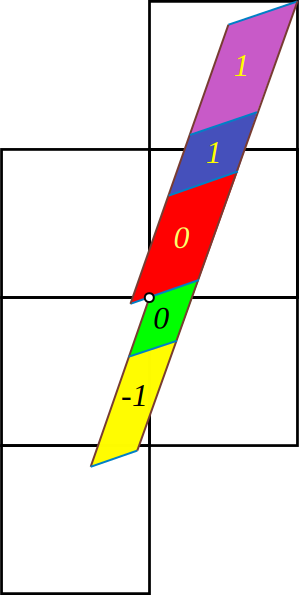
\includegraphics[width=1.0\textwidth]{PVAdlerWeissB-b}\\(b)
%            \end{center}\end{minipage}
%            \begin{minipage}[c]{0.23\textwidth}\begin{center}
%\includegraphics[width=1.0\textwidth]{PVAdlerWeissB-c}\\(c)
%            \end{center}\end{minipage}
%\end{center}
%%%%%%%%%%%%%%%%%%%%%%%%%%%%%%%%%%%%%%%%%%%%%%%%%%%%%%%%%%%%%%%%
%(b)
%mapped step forward in time, the rectangles are stretched along the
%unstable direction and shrunk along the stable direction
%
%(c) sub-rectangles
%$\pS_j$ that have to be translated back into the partition are indicated by
%color and labeled by their lattice translations
%$\Ssym{j}\in\A=\{\underline{1},0,1\}$
%%%%%%%%%%%%%%%%%%%%%%%%%%%%%%%%%%%%%%%%%%%%%%%%%%%%%%%%%%%%%%%%
%\end{frame} %%%%%%%%%%%%%%%%%%%%%%%%%%%%%%%%%%%%%%%%%%%%%%

%\begin{frame}{cat map generating partition}
%%%%%%%%%%%%%%%%%%%%%%%%%%%%%%%%%%%%%%%%%%%%%%%%%%%%%%%%%%%%%%
%% PC 2018-02-09 from siminos/cats/catAdlerWeiss.tex
%% \caption{\label{fig:PVAdlerWeissB}
%\begin{center}
%            \begin{minipage}[c]{0.23\textwidth}\begin{center}
%\includegraphics[width=1.0\textwidth]{PVAdlerWeissB-a}\\(a)
%            \end{center}\end{minipage}
%%            \begin{minipage}[c]{0.23\textwidth}\begin{center}
%%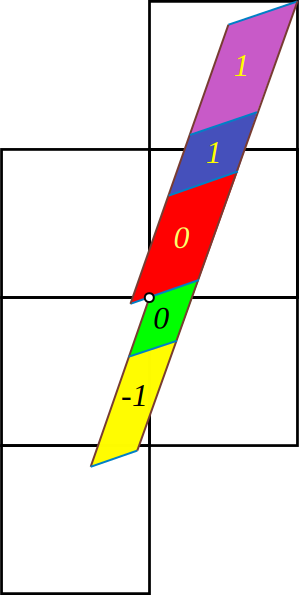
\includegraphics[width=1.0\textwidth]{PVAdlerWeissB-b}\\(b)
%%            \end{center}\end{minipage}
%            \begin{minipage}[c]{0.23\textwidth}\begin{center}
%\includegraphics[width=1.0\textwidth]{PVAdlerWeissB-c}\\(c)
%            \end{center}\end{minipage}
%            ~~~
%            \begin{minipage}[c]{0.09\textwidth}\begin{center}
%\includegraphics[width=1.0\textwidth]{PVAWMarkovCol}\\(d)
%            \end{center}\end{minipage}
%\end{center}
%%%%%%%%%%%%%%%%%%%%%%%%%%%%%%%%%%%%%%%%%%%%%%%%%%%%%%%%%%%%%%%%
%(c)
%sub-rectangles $\pS_j$ yield a generating partition, with
%\\
%(d)
%the finite grammar given by the finite {\markGraph}.
%
%%\medskip
%%
%%The nodes
%%refer to the rectangles $A$ and $B$, \\
%%the five links correspond to the five sub-rectangles \\
%%induced by one step forward-time dynamics.
%%%\footnote{For details, see ChaosBook.org}
%
%%\vfill
%%\bigskip {\scriptsize \em
%%\hfill \textcolor{green}{this construction is new, not in literature}
%%         }
%\end{frame} %%%%%%%%%%%%%%%%%%%%%%%%%%%%%%%%%%%%%%%%%%%%%%

%\begin{frame}{cat map Perron-Frobenious operator}
%%%%%%%%%%%%%%%%%%%%%%%%%%%%%%%%%%%%%%%%%%%%%%%%%%%%%%%%%%%%%%
%% PC 2018-02-09 from siminos/cats/catAdlerWeiss.tex
%% \caption{\label{fig:PVAdlerWeissB}
%\begin{center}
%            \begin{minipage}[c]{0.23\textwidth}\begin{center}
%\includegraphics[width=1.0\textwidth]{PVAdlerWeissB-a}
%            \end{center}\end{minipage}
%            \begin{minipage}[c]{0.23\textwidth}\begin{center}
%\includegraphics[width=1.0\textwidth]{PVAdlerWeissB-c}
%            \end{center}\end{minipage}
%            ~~~
%            \begin{minipage}[c]{0.09\textwidth}\begin{center}
%\includegraphics[width=1.0\textwidth]{PVAWMarkovCol}
%            \end{center}\end{minipage}
%\end{center}
%%%%%%%%%%%%%%%%%%%%%%%%%%%%%%%%%%%%%%%%%%%%%%%%%%%%%%%%%%%%%%
%% PC 2018-02-09 from siminos/spatiotemp/chapter/blogHL.tex
%the two-rectangle partition has [2$\times$2] Markov
%matrix, \\ where one sums over all admissible transitions:
%\bea
%\left[\begin{array}{c} \phi'_A \\ \phi'_B \end{array}\right]
%&=& L\phi =
%\left[
%\begin{array}{cc}
% L_{A{}^0\!A}+L_{A{}^1\!A} & L_{A{}^{\underline{1}}\!B} \\
% L_{B{}^1\!A} & L_{B{}^0\!B} \\
%\end{array}
%\right]
%\left[\begin{array}{c} \phi_A \\ \phi_B \end{array}\right]
%    \continue       %{2rectTransfMatrEq}
%L &=&
%\frac{1}{\ExpaEig}
%\left[\begin{array}{cc}
% 2          & \ExpaEig-2 \\
% \ExpaEig-1 & 1          \\
%\end{array}\right]
%\nnu %\label{2rectTransfMatrEq1}
%\eea
%%%%%%%%%%%%%%%%%%%%%%%%%%%%%%%%%%%%%%%%%%%%%%%%%%%%%%%%%%%%%%%%
%\end{frame} %%%%%%%%%%%%%%%%%%%%%%%%%%%%%%%%%%%%%%%%%%%%%%

%\begin{frame}{cat map dynamical zeta function}
%%%%%%%%%%%%%%%%%%%%%%%%%%%%%%%%%%%%%%%%%%%%%%%%%%%%%%%%%%%%%%
%% PC 2018-02-09 from siminos/cats/catAdlerWeiss.tex
%% \caption{\label{fig:PVAdlerWeissB}
%\begin{center}
%            \begin{minipage}[c]{0.23\textwidth}\begin{center}
%\includegraphics[width=1.0\textwidth]{PVAdlerWeissB-a}
%            \end{center}\end{minipage}
%            \begin{minipage}[c]{0.23\textwidth}\begin{center}
%\includegraphics[width=1.0\textwidth]{PVAdlerWeissB-c}
%            \end{center}\end{minipage}
%            ~~~
%            \begin{minipage}[c]{0.09\textwidth}\begin{center}
%\includegraphics[width=1.0\textwidth]{PVAWMarkovCol}
%            \end{center}\end{minipage}
%\end{center}
%%%%%%%%%%%%%%%%%%%%%%%%%%%%%%%%%%%%%%%%%%%%%%%%%%%%%%%%%%%%%%
%% PC 2018-02-09 from siminos/spatiotemp/chapter/blogHL.tex
%every long-time property of cat maps dynamics is encoded in \\
%the Fredholm determinant \\
%(topological zeta function\footfullcite{Isola90};
%Markov graph determinant)
%\[
%\det(1-zL) = %2019-01-03 PC no longer understands where
%             %           the commented-out version came from....
% % 1-3\frac{z}{\ExpaEig}
% %   -\frac{z^2}{\ExpaEig}(\ExpaEig-3)
% \frac{1 - 3 z + z^2}{(1 - z)^2}
%%\label{2rectDetTransfMatr}
%\]
%%%%%%%%%%%%%%%%%%%%%%%%%%%%%%%%%%%%%%%%%%%%%%%%%%%%%%%%%%%%%%%%
%
%{\Huge \textcolor{red}{solved!}} \hfill every expectation value computable
%\end{frame} %%%%%%%%%%%%%%%%%%%%%%%%%%%%%%%%%%%%%%%%%%%%%%


\end{document}
